\documentclass[]{scrartcl}
\usepackage[left=1in,top=1in,right=1in,bottom=1in]{geometry}
\newcommand*{\authorfont}{\fontfamily{phv}\selectfont}
\usepackage{epigrafica}


  \usepackage[T1]{fontenc}
  \usepackage[utf8]{inputenc}

\usepackage{graphicx}
%\usepackage{subfig}
\usepackage{subcaption}
\usepackage{pdflscape}
\usepackage{longtable}
\usepackage{booktabs}

\usepackage{epigrafica}
	\renewcommand{\sfdefault}{txss}
	\renewcommand{\familydefault}
	{\sfdefault}

\usepackage{abstract}
\renewcommand{\abstractname}{Report summary}    % clear the title
\renewcommand{\absnamepos}{left} % originally center

\renewenvironment{abstract}
 {{%
    \setlength{\leftmargin}{0mm}
    \setlength{\rightmargin}{\leftmargin}%
  }%
  \relax}
 {\endlist}

\makeatletter
\def\@maketitle{%
  \newpage
%  \null
%  \vskip 2em%
%  \begin{center}%
  \let \footnote \thanks
    {\fontsize{18}{20}\selectfont\raggedright  \setlength{\parindent}{0pt} \@title \par}%
}
%\fi
\makeatother



\def\tightlist{}

\setcounter{secnumdepth}{0}

\usepackage{color}
\usepackage{fancyvrb}
\newcommand{\VerbBar}{|}
\newcommand{\VERB}{\Verb[commandchars=\\\{\}]}
\DefineVerbatimEnvironment{Highlighting}{Verbatim}{commandchars=\\\{\}}
% Add ',fontsize=\small' for more characters per line
\usepackage{framed}
\definecolor{shadecolor}{RGB}{248,248,248}
\newenvironment{Shaded}{\begin{snugshade}}{\end{snugshade}}
\newcommand{\AlertTok}[1]{\textcolor[rgb]{0.94,0.16,0.16}{#1}}
\newcommand{\AnnotationTok}[1]{\textcolor[rgb]{0.56,0.35,0.01}{\textbf{\textit{#1}}}}
\newcommand{\AttributeTok}[1]{\textcolor[rgb]{0.77,0.63,0.00}{#1}}
\newcommand{\BaseNTok}[1]{\textcolor[rgb]{0.00,0.00,0.81}{#1}}
\newcommand{\BuiltInTok}[1]{#1}
\newcommand{\CharTok}[1]{\textcolor[rgb]{0.31,0.60,0.02}{#1}}
\newcommand{\CommentTok}[1]{\textcolor[rgb]{0.56,0.35,0.01}{\textit{#1}}}
\newcommand{\CommentVarTok}[1]{\textcolor[rgb]{0.56,0.35,0.01}{\textbf{\textit{#1}}}}
\newcommand{\ConstantTok}[1]{\textcolor[rgb]{0.00,0.00,0.00}{#1}}
\newcommand{\ControlFlowTok}[1]{\textcolor[rgb]{0.13,0.29,0.53}{\textbf{#1}}}
\newcommand{\DataTypeTok}[1]{\textcolor[rgb]{0.13,0.29,0.53}{#1}}
\newcommand{\DecValTok}[1]{\textcolor[rgb]{0.00,0.00,0.81}{#1}}
\newcommand{\DocumentationTok}[1]{\textcolor[rgb]{0.56,0.35,0.01}{\textbf{\textit{#1}}}}
\newcommand{\ErrorTok}[1]{\textcolor[rgb]{0.64,0.00,0.00}{\textbf{#1}}}
\newcommand{\ExtensionTok}[1]{#1}
\newcommand{\FloatTok}[1]{\textcolor[rgb]{0.00,0.00,0.81}{#1}}
\newcommand{\FunctionTok}[1]{\textcolor[rgb]{0.00,0.00,0.00}{#1}}
\newcommand{\ImportTok}[1]{#1}
\newcommand{\InformationTok}[1]{\textcolor[rgb]{0.56,0.35,0.01}{\textbf{\textit{#1}}}}
\newcommand{\KeywordTok}[1]{\textcolor[rgb]{0.13,0.29,0.53}{\textbf{#1}}}
\newcommand{\NormalTok}[1]{#1}
\newcommand{\OperatorTok}[1]{\textcolor[rgb]{0.81,0.36,0.00}{\textbf{#1}}}
\newcommand{\OtherTok}[1]{\textcolor[rgb]{0.56,0.35,0.01}{#1}}
\newcommand{\PreprocessorTok}[1]{\textcolor[rgb]{0.56,0.35,0.01}{\textit{#1}}}
\newcommand{\RegionMarkerTok}[1]{#1}
\newcommand{\SpecialCharTok}[1]{\textcolor[rgb]{0.00,0.00,0.00}{#1}}
\newcommand{\SpecialStringTok}[1]{\textcolor[rgb]{0.31,0.60,0.02}{#1}}
\newcommand{\StringTok}[1]{\textcolor[rgb]{0.31,0.60,0.02}{#1}}
\newcommand{\VariableTok}[1]{\textcolor[rgb]{0.00,0.00,0.00}{#1}}
\newcommand{\VerbatimStringTok}[1]{\textcolor[rgb]{0.31,0.60,0.02}{#1}}
\newcommand{\WarningTok}[1]{\textcolor[rgb]{0.56,0.35,0.01}{\textbf{\textit{#1}}}}

%%\usepackage{graphicx}
% We will generate all images so they have a width \maxwidth. This means
% that they will get their normal width if they fit onto the page, but
% are scaled down if they would overflow the margins.
%\makeatletter
%\def\maxwidth{\ifdim\Gin@nat@width>\linewidth\linewidth
%\else\Gin@nat@width\fi}
%\makeatother
%\let\Oldincludegraphics\includegraphics
%\renewcommand{\includegraphics}[1]{\Oldincludegraphics[width=\maxwidth]{#1}}
%
\title{Supplementary information \newline \\ \Large \emph{Data plots \& R script}   }

\date{2020-10-18}





\author{\Large DA McGranahan  \normalsize \emph{School of Natural Resource Sciences, Range Science; North Dakota State
University, Fargo, ND}   \and \Large BN Poling  \normalsize \emph{School of Natural Resource Sciences, Range Science; North Dakota State
University, Fargo, ND}  }


% \usepackage{titlesec}




\newtheorem{hypothesis}{Hypothesis}
\usepackage{setspace}

\makeatletter
\@ifpackageloaded{hyperref}{}{%
\ifxetex
  \usepackage[setpagesize=false, % page size defined by xetex
              unicode=false, % unicode breaks when used with xetex
              xetex]{hyperref}
\else
  \usepackage[unicode=true]{hyperref}
\fi
}
\@ifpackageloaded{color}{
    \PassOptionsToPackage{usenames,dvipsnames}{color}
}{%
    \usepackage[usenames,dvipsnames]{color}
}
\makeatother
\hypersetup{breaklinks=true,
            bookmarks=true,
            pdfauthor={DA McGranahan (School of Natural Resource Sciences, Range Science; North Dakota State
University, Fargo, ND) and BN Poling (School of Natural Resource Sciences, Range Science; North Dakota State
University, Fargo, ND)},
             pdfkeywords = {},  
            pdftitle={Supplementary information: Data plots \& R script},
            colorlinks=true,
            citecolor=blue,
            urlcolor=blue,
            linkcolor=magenta,
            pdfborder={0 0 0}}
\urlstyle{same}  % don't use monospace font for urls



\begin{document}
	
% \pagenumbering{arabic}% resets `page` counter to 1 
%
% \maketitle

{% \usefont{T1}{pnc}{m}{n}
\setlength{\parindent}{0pt}
\thispagestyle{plain}
{\fontsize{18}{20}\selectfont\raggedright 
\maketitle  % title \par  
}


{
   \vskip 13.5pt\relax \normalsize\fontsize{11}{12} 
\textbf{\authorfont DA McGranahan} \newline \hspace{0.1in} \vspace{0.05in}  \emph{\small School of Natural Resource Sciences, Range Science; North Dakota State
University, Fargo, ND}   \par \textbf{\authorfont BN Poling} \newline \hspace{0.1in} \vspace{0.05in}  \emph{\small School of Natural Resource Sciences, Range Science; North Dakota State
University, Fargo, ND}   

}

}


\date{}



\vskip 6.5pt

\noindent  \newpage

\hypertarget{annual-crops}{%
\section{Annual crops}\label{annual-crops}}

\hypertarget{raw-data}{%
\subsection{Raw data}\label{raw-data}}

\begin{figure}[!h]
  \centering
  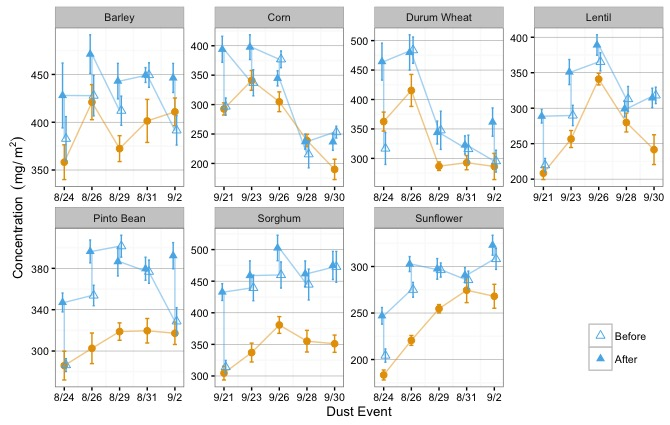
\includegraphics[width=0.9\textwidth]{figures/chlorconc.jpg}\\
  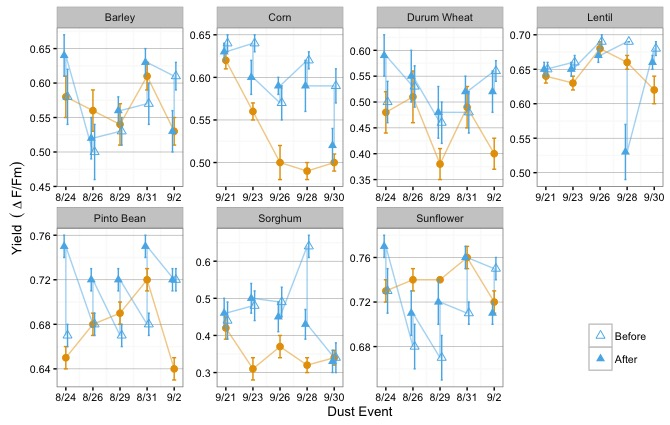
\includegraphics[width=0.9\textwidth]{figures/photoact.jpg}\\
  \caption{\textbf{TOP:} Chlorophyll concentration; \textbf{BOTTOM:} Photosynthetic yield. }
\end{figure}

\clearpage

\begin{figure}[!h]
  \centering
  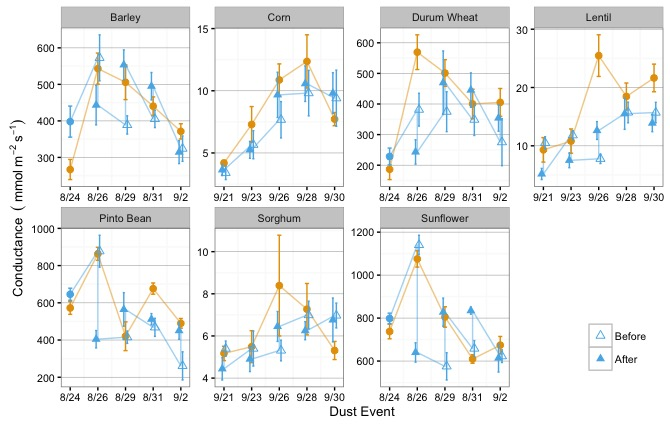
\includegraphics[width=0.9\textwidth]{figures/stomcond.jpg}\\
  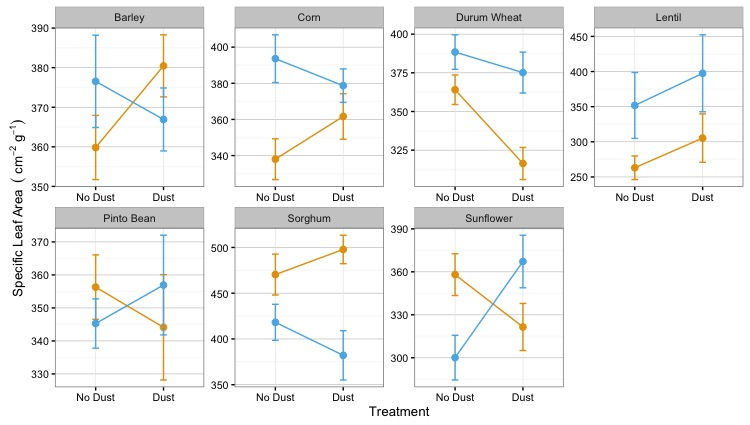
\includegraphics[width=0.9\textwidth]{figures/SLA.jpg}
  \caption{\textbf{TOP:} Stomatal conductance; \textbf{BOTTOM:} Specific leaf area. }
\end{figure}

\clearpage

\hypertarget{short-term-responses}{%
\subsection{Short-term responses}\label{short-term-responses}}

\begin{figure}
\centering
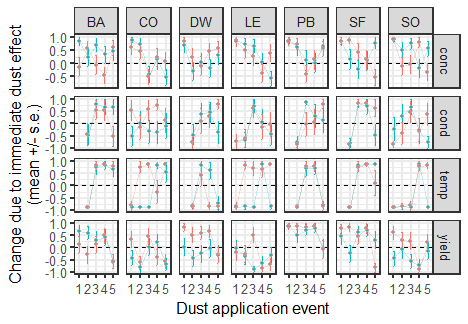
\includegraphics{figures/diff_gg-1.png}
\caption{Immediate changes (after dusting values - pre-dusting values)
in three physiological responses among 7 annual crop species over 5 dust
application events that occurred 3 days apart. Colors indicate two
blocks on different greenhouse benches.}
\end{figure}

\begin{table}[ht]
\centering
\begin{tabular}{lrrrrrrrr}
  \hline
 & Df & AIC & BIC & logLik & deviance & Chisq & Chi Df & Pr($>$Chisq) \\ 
  \hline
diff0 & 2 & 3817.2 & 3827.6 & -1906.6 & 3813.2 &  &  &  \\ 
  diff1 & 5 & 3783.2 & 3809.3 & -1886.6 & 3773.2 & 39.9 & 3 & 0.000 \\ 
   \hline
\end{tabular}
\caption{Immediate physiological responses to dusting vary among response measurements.} 
\end{table}

\clearpage

\hypertarget{perennial-grasses}{%
\section{Perennial Grasses}\label{perennial-grasses}}

\begin{figure}[!h]
  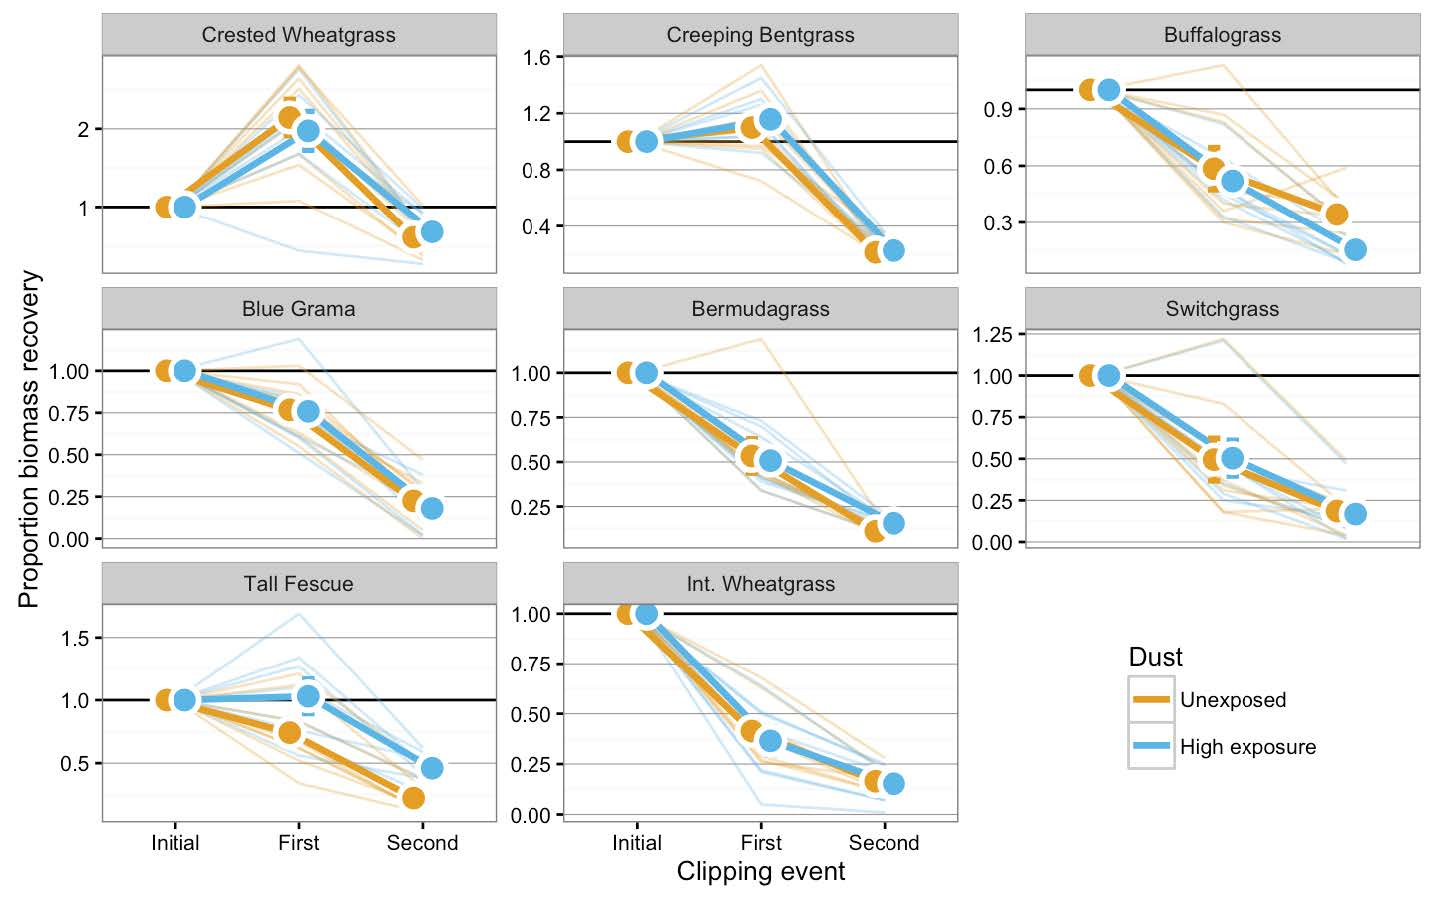
\includegraphics[width=1\textwidth]{figures/grassrecovery.jpg}
  \caption{Biomass recovery for eight perennial grasses following two rounds of clipping under dusted and undusted conditions. }
\end{figure}

\clearpage

\hypertarget{r-script}{%
\section{R script}\label{r-script}}

\begin{Shaded}
\begin{Highlighting}[]
\CommentTok{#}
\CommentTok{# Annual crops }
\CommentTok{#}
\CommentTok{#}
\CommentTok{# Short-term responses}
\CommentTok{#}
\CommentTok{#}
\CommentTok{# Regresion modelling }
\CommentTok{#}
\CommentTok{# Model fitting }
\CommentTok{#}
\CommentTok{# Responses by species }
\CommentTok{#}
  \CommentTok{# Chlorophyll concentration  }
\NormalTok{    conc0 <-}\StringTok{ }\NormalTok{lme4}\OperatorTok{::}\KeywordTok{lmer}\NormalTok{(diff }\OperatorTok{~}\StringTok{ }\DecValTok{0} \OperatorTok{+}\StringTok{ }\NormalTok{(}\DecValTok{1}\OperatorTok{|}\NormalTok{block}\OperatorTok{:}\NormalTok{round}\OperatorTok{:}\NormalTok{pot), }\DataTypeTok{REML =}\NormalTok{ F,}
                        \DataTypeTok{data =} \KeywordTok{filter}\NormalTok{(diff_dat, response }\OperatorTok{==}\StringTok{ "conc"}\NormalTok{)) }
\NormalTok{    conc1 <-}\StringTok{ }\NormalTok{lme4}\OperatorTok{::}\KeywordTok{lmer}\NormalTok{(diff }\OperatorTok{~}\StringTok{ }\DecValTok{0} \OperatorTok{+}\StringTok{ }\NormalTok{spp }\OperatorTok{+}\StringTok{ }\NormalTok{(}\DecValTok{1}\OperatorTok{|}\NormalTok{block}\OperatorTok{:}\NormalTok{round}\OperatorTok{:}\NormalTok{pot), }\DataTypeTok{REML =}\NormalTok{ F,}
                        \DataTypeTok{data =} \KeywordTok{filter}\NormalTok{(diff_dat, response }\OperatorTok{==}\StringTok{ "conc"}\NormalTok{)) }

\NormalTok{    conc_diff_CI <-}\StringTok{ }\KeywordTok{as.data.frame}\NormalTok{(}\KeywordTok{confint}\NormalTok{(conc1)) }\OperatorTok
\StringTok{                      }\KeywordTok{rownames_to_column}\NormalTok{(}\StringTok{"term"}\NormalTok{) }\OperatorTok
\StringTok{                      }\KeywordTok{slice}\NormalTok{(}\OperatorTok{-}\NormalTok{(}\DecValTok{1}\OperatorTok{:}\DecValTok{2}\NormalTok{)) }\OperatorTok
\StringTok{                      }\KeywordTok{bind_cols}\NormalTok{(}\KeywordTok{tibble}\NormalTok{(}
                        \DataTypeTok{estimate =}\NormalTok{ lme4}\OperatorTok{::}\KeywordTok{fixef}\NormalTok{(conc1), }
                        \DataTypeTok{response =} \StringTok{"Chlorophyll}\CharTok{\textbackslash{}n}\StringTok{concentration"}\NormalTok{) ) }
  \CommentTok{# Stomatal conductance}
\NormalTok{    cond0 <-}\StringTok{ }\NormalTok{lme4}\OperatorTok{::}\KeywordTok{lmer}\NormalTok{(diff }\OperatorTok{~}\StringTok{ }\DecValTok{0} \OperatorTok{+}\StringTok{ }\NormalTok{(}\DecValTok{1}\OperatorTok{|}\NormalTok{block}\OperatorTok{:}\NormalTok{round}\OperatorTok{:}\NormalTok{pot), }\DataTypeTok{REML =}\NormalTok{ F,}
                        \DataTypeTok{data =} \KeywordTok{filter}\NormalTok{(diff_dat, response }\OperatorTok{==}\StringTok{ "cond"}\NormalTok{)) }
\NormalTok{    cond1 <-}\StringTok{ }\NormalTok{lme4}\OperatorTok{::}\KeywordTok{lmer}\NormalTok{(diff }\OperatorTok{~}\StringTok{ }\DecValTok{0} \OperatorTok{+}\StringTok{ }\NormalTok{spp }\OperatorTok{+}\StringTok{ }\NormalTok{(}\DecValTok{1}\OperatorTok{|}\NormalTok{block}\OperatorTok{:}\NormalTok{round}\OperatorTok{:}\NormalTok{pot), }\DataTypeTok{REML =}\NormalTok{ F,}
                        \DataTypeTok{data =} \KeywordTok{filter}\NormalTok{(diff_dat, response }\OperatorTok{==}\StringTok{ "cond"}\NormalTok{)) }
    
\NormalTok{    cond_diff_CI <-}\StringTok{ }\KeywordTok{as.data.frame}\NormalTok{(}\KeywordTok{confint}\NormalTok{(cond1)) }\OperatorTok
\StringTok{                      }\KeywordTok{rownames_to_column}\NormalTok{(}\StringTok{"term"}\NormalTok{) }\OperatorTok
\StringTok{                      }\KeywordTok{slice}\NormalTok{(}\OperatorTok{-}\NormalTok{(}\DecValTok{1}\OperatorTok{:}\DecValTok{2}\NormalTok{)) }\OperatorTok
\StringTok{                      }\KeywordTok{bind_cols}\NormalTok{(}\KeywordTok{tibble}\NormalTok{(}
                        \DataTypeTok{estimate =}\NormalTok{ lme4}\OperatorTok{::}\KeywordTok{fixef}\NormalTok{(cond1), }
                        \DataTypeTok{response =} \StringTok{"Stomatal}\CharTok{\textbackslash{}n}\StringTok{conductance"}\NormalTok{) ) }
  \CommentTok{# Photosynthetic yield}
\NormalTok{    yield0 <-}\StringTok{ }\NormalTok{lme4}\OperatorTok{::}\KeywordTok{lmer}\NormalTok{(diff }\OperatorTok{~}\StringTok{ }\DecValTok{0} \OperatorTok{+}\StringTok{ }\NormalTok{(}\DecValTok{1}\OperatorTok{|}\NormalTok{block}\OperatorTok{:}\NormalTok{round}\OperatorTok{:}\NormalTok{pot), }\DataTypeTok{REML =}\NormalTok{ F,}
                        \DataTypeTok{data =} \KeywordTok{filter}\NormalTok{(diff_dat, response }\OperatorTok{==}\StringTok{ "yield"}\NormalTok{)) }
\NormalTok{    yield1 <-}\StringTok{ }\NormalTok{lme4}\OperatorTok{::}\KeywordTok{lmer}\NormalTok{(diff }\OperatorTok{~}\StringTok{ }\DecValTok{0} \OperatorTok{+}\StringTok{ }\NormalTok{spp }\OperatorTok{+}\StringTok{ }\NormalTok{(}\DecValTok{1}\OperatorTok{|}\NormalTok{block}\OperatorTok{:}\NormalTok{round}\OperatorTok{:}\NormalTok{pot), }\DataTypeTok{REML =}\NormalTok{ F,}
                        \DataTypeTok{data =} \KeywordTok{filter}\NormalTok{(diff_dat, response }\OperatorTok{==}\StringTok{ "yield"}\NormalTok{)) }
    
\NormalTok{    yield_diff_CI <-}\StringTok{ }\KeywordTok{as.data.frame}\NormalTok{(}\KeywordTok{confint}\NormalTok{(yield1)) }\OperatorTok
\StringTok{                      }\KeywordTok{rownames_to_column}\NormalTok{(}\StringTok{"term"}\NormalTok{) }\OperatorTok
\StringTok{                      }\KeywordTok{slice}\NormalTok{(}\OperatorTok{-}\NormalTok{(}\DecValTok{1}\OperatorTok{:}\DecValTok{2}\NormalTok{)) }\OperatorTok
\StringTok{                      }\KeywordTok{bind_cols}\NormalTok{(}\KeywordTok{tibble}\NormalTok{(}
                        \DataTypeTok{estimate =}\NormalTok{ lme4}\OperatorTok{::}\KeywordTok{fixef}\NormalTok{(yield1), }
                        \DataTypeTok{response =} \StringTok{"Photosynthetic}\CharTok{\textbackslash{}n}\StringTok{yield"}\NormalTok{) ) }
\NormalTok{    diffCIs <-}\StringTok{ }\KeywordTok{bind_rows}\NormalTok{(cond_diff_CI, }
\NormalTok{                        conc_diff_CI, }
\NormalTok{                        yield_diff_CI) }
    \KeywordTok{colnames}\NormalTok{(diffCIs) <-}\StringTok{ }\KeywordTok{c}\NormalTok{(}\StringTok{"term"}\NormalTok{, }\StringTok{"ciL"}\NormalTok{, }\StringTok{"ciU"}\NormalTok{, }\StringTok{"estimate"}\NormalTok{, }\StringTok{"response"}\NormalTok{)}
\CommentTok{#}
\CommentTok{# Overall responses}
\CommentTok{#}
\NormalTok{    diff0 <-}\StringTok{ }\NormalTok{lme4}\OperatorTok{::}\KeywordTok{lmer}\NormalTok{(diff }\OperatorTok{~}\StringTok{ }\DecValTok{0} \OperatorTok{+}\StringTok{ }\NormalTok{(}\DecValTok{1}\OperatorTok{|}\NormalTok{block}\OperatorTok{:}\NormalTok{round}\OperatorTok{:}\NormalTok{spp), }
                        \DataTypeTok{data=}\NormalTok{ diff_dat, }\DataTypeTok{REML =}\NormalTok{ F) }
\NormalTok{    diff1 <-}\StringTok{ }\NormalTok{lme4}\OperatorTok{::}\KeywordTok{lmer}\NormalTok{(diff }\OperatorTok{~}\StringTok{ }\DecValTok{0} \OperatorTok{+}\StringTok{ }\NormalTok{response }\OperatorTok{+}\StringTok{ }\NormalTok{(}\DecValTok{1}\OperatorTok{|}\NormalTok{block}\OperatorTok{:}\NormalTok{round}\OperatorTok{:}\NormalTok{spp), }
                        \DataTypeTok{data=}\NormalTok{ diff_dat, }\DataTypeTok{REML =}\NormalTok{ F) }
\NormalTok{    dmc <-}\StringTok{ }\KeywordTok{anova}\NormalTok{(diff0, diff1)}

\NormalTok{    diff_CI <-}\StringTok{ }\KeywordTok{as.data.frame}\NormalTok{(}\KeywordTok{confint}\NormalTok{(diff1)) }\OperatorTok
\StringTok{                }\KeywordTok{rownames_to_column}\NormalTok{(}\StringTok{"term"}\NormalTok{) }\OperatorTok
\StringTok{                }\KeywordTok{slice}\NormalTok{(}\OperatorTok{-}\NormalTok{(}\DecValTok{1}\OperatorTok{:}\DecValTok{2}\NormalTok{)) }\OperatorTok
\StringTok{                }\KeywordTok{bind_cols}\NormalTok{(}\KeywordTok{tibble}\NormalTok{(}
                  \DataTypeTok{estimate =}\NormalTok{ lme4}\OperatorTok{::}\KeywordTok{fixef}\NormalTok{(diff1)) )}
    \KeywordTok{colnames}\NormalTok{(diff_CI) <-}\StringTok{ }\KeywordTok{c}\NormalTok{(}\StringTok{"term"}\NormalTok{, }\StringTok{"ciL"}\NormalTok{, }\StringTok{"ciU"}\NormalTok{, }\StringTok{"estimate"}\NormalTok{)}
\CommentTok{#}
\CommentTok{#  Long-term responses}
\CommentTok{#}
\CommentTok{# Mixed-effect model fitting}
  \CommentTok{# Specific leaf area}
\NormalTok{    sla.null <-}\StringTok{ }\NormalTok{lme4}\OperatorTok{::}\KeywordTok{lmer}\NormalTok{(}\KeywordTok{scale}\NormalTok{(}\KeywordTok{log}\NormalTok{(SLA)) }\OperatorTok{~}\StringTok{ }\DecValTok{1} \OperatorTok{+}\StringTok{ }\NormalTok{(}\DecValTok{1}\OperatorTok{|}\NormalTok{block), }
                           \DataTypeTok{data=}\NormalTok{SLA2, }\DataTypeTok{REML=}\OtherTok{FALSE}\NormalTok{)}
\NormalTok{    sla.spp <-}\StringTok{ }\NormalTok{lme4}\OperatorTok{::}\KeywordTok{lmer}\NormalTok{(}\KeywordTok{scale}\NormalTok{(}\KeywordTok{log}\NormalTok{(SLA)) }\OperatorTok{~}\StringTok{ }\NormalTok{spp }\OperatorTok{+}\StringTok{ }\NormalTok{(}\DecValTok{1}\OperatorTok{|}\NormalTok{block), }
                          \DataTypeTok{data=}\NormalTok{SLA2, }\DataTypeTok{REML=}\OtherTok{FALSE}\NormalTok{)}
\NormalTok{    sla.treat <-}\StringTok{ }\NormalTok{lme4}\OperatorTok{::}\KeywordTok{lmer}\NormalTok{(}\KeywordTok{scale}\NormalTok{(}\KeywordTok{log}\NormalTok{(SLA)) }\OperatorTok{~}\StringTok{ }\NormalTok{t_c }\OperatorTok{+}\StringTok{ }\NormalTok{(}\DecValTok{1}\OperatorTok{|}\NormalTok{block), }
                            \DataTypeTok{data=}\NormalTok{SLA2, }\DataTypeTok{REML=}\OtherTok{FALSE}\NormalTok{)}
\NormalTok{    sla.add <-}\StringTok{ }\NormalTok{lme4}\OperatorTok{::}\KeywordTok{lmer}\NormalTok{(}\KeywordTok{scale}\NormalTok{(}\KeywordTok{log}\NormalTok{(SLA)) }\OperatorTok{~}\StringTok{ }\DecValTok{0} \OperatorTok{+}\StringTok{ }\NormalTok{spp }\OperatorTok{+}\StringTok{ }\NormalTok{t_c }\OperatorTok{+}\StringTok{ }\NormalTok{(}\DecValTok{1}\OperatorTok{|}\NormalTok{block), }
                          \DataTypeTok{data=}\NormalTok{SLA2, }\DataTypeTok{REML=}\OtherTok{FALSE}\NormalTok{)}
\NormalTok{    sla.int <-}\StringTok{ }\NormalTok{lme4}\OperatorTok{::}\KeywordTok{lmer}\NormalTok{(}\KeywordTok{scale}\NormalTok{(}\KeywordTok{log}\NormalTok{(SLA)) }\OperatorTok{~}\StringTok{ }\DecValTok{0} \OperatorTok{+}\StringTok{ }\NormalTok{spp }\OperatorTok{*}\StringTok{ }\NormalTok{t_c }\OperatorTok{+}\StringTok{ }\NormalTok{(}\DecValTok{1}\OperatorTok{|}\NormalTok{block), }
                          \DataTypeTok{data=}\NormalTok{SLA2, }\DataTypeTok{REML=}\OtherTok{FALSE}\NormalTok{)}
  \CommentTok{# Stomatal conductance}
\NormalTok{    conduct.null <-}\StringTok{ }\NormalTok{lme4}\OperatorTok{::}\KeywordTok{lmer}\NormalTok{(}\KeywordTok{scale}\NormalTok{(lcond) }\OperatorTok{~}\StringTok{ }\DecValTok{1} \OperatorTok{+}\StringTok{ }\NormalTok{(}\DecValTok{1}\OperatorTok{|}\NormalTok{block}\OperatorTok{:}\NormalTok{date}\OperatorTok{:}\NormalTok{pot),}
                               \DataTypeTok{data=}\NormalTok{Por, }\DataTypeTok{REML=}\OtherTok{FALSE}\NormalTok{)}
\NormalTok{    conduct.spp <-}\StringTok{ }\NormalTok{lme4}\OperatorTok{::}\KeywordTok{lmer}\NormalTok{(}\KeywordTok{scale}\NormalTok{(lcond) }\OperatorTok{~}\StringTok{ }\NormalTok{spp }\OperatorTok{+}\StringTok{ }\NormalTok{(}\DecValTok{1}\OperatorTok{|}\NormalTok{block}\OperatorTok{:}\NormalTok{date}\OperatorTok{:}\NormalTok{pot), }
                              \DataTypeTok{data=}\NormalTok{Por, }\DataTypeTok{REML=}\OtherTok{FALSE}\NormalTok{)}
\NormalTok{    conduct.treat <-}\StringTok{ }\NormalTok{lme4}\OperatorTok{::}\KeywordTok{lmer}\NormalTok{(}\KeywordTok{scale}\NormalTok{(lcond) }\OperatorTok{~}\StringTok{ }\NormalTok{t_c }\OperatorTok{+}\StringTok{ }\NormalTok{(}\DecValTok{1}\OperatorTok{|}\NormalTok{block}\OperatorTok{:}\NormalTok{date}\OperatorTok{:}\NormalTok{pot), }
                                \DataTypeTok{data=}\NormalTok{Por, }\DataTypeTok{REML=}\OtherTok{FALSE}\NormalTok{)}
\NormalTok{    conduct.add <-}\StringTok{ }\NormalTok{lme4}\OperatorTok{::}\KeywordTok{lmer}\NormalTok{(}\KeywordTok{scale}\NormalTok{(lcond) }\OperatorTok{~}\StringTok{ }\DecValTok{0} \OperatorTok{+}\StringTok{ }\NormalTok{spp }\OperatorTok{+}\StringTok{ }\NormalTok{t_c }\OperatorTok{+}\StringTok{ }\NormalTok{(}\DecValTok{1}\OperatorTok{|}\NormalTok{block}\OperatorTok{:}\NormalTok{date}\OperatorTok{:}\NormalTok{pot), }
                              \DataTypeTok{data=}\NormalTok{Por, }\DataTypeTok{REML=}\OtherTok{FALSE}\NormalTok{)}
\NormalTok{    conduct.int <-}\StringTok{ }\NormalTok{lme4}\OperatorTok{::}\KeywordTok{lmer}\NormalTok{(}\KeywordTok{scale}\NormalTok{(lcond) }\OperatorTok{~}\StringTok{ }\DecValTok{0} \OperatorTok{+}\StringTok{ }\NormalTok{spp }\OperatorTok{*}\StringTok{ }\NormalTok{t_c  }\OperatorTok{+}\StringTok{ }\NormalTok{(}\DecValTok{1}\OperatorTok{|}\NormalTok{block}\OperatorTok{:}\NormalTok{date}\OperatorTok{:}\NormalTok{pot), }
                              \DataTypeTok{data=}\NormalTok{Por, }\DataTypeTok{REML=}\OtherTok{FALSE}\NormalTok{)}
  \CommentTok{# Chlorophyll content}
\NormalTok{    conc.null <-}\StringTok{ }\NormalTok{lme4}\OperatorTok{::}\KeywordTok{lmer}\NormalTok{(}\KeywordTok{scale}\NormalTok{(lconc) }\OperatorTok{~}\StringTok{ }\DecValTok{1} \OperatorTok{+}\StringTok{ }\NormalTok{(}\DecValTok{1}\OperatorTok{|}\NormalTok{block}\OperatorTok{:}\NormalTok{date}\OperatorTok{:}\NormalTok{pot), }
                            \DataTypeTok{data=}\NormalTok{CCM2, }\DataTypeTok{REML=}\OtherTok{FALSE}\NormalTok{)}
\NormalTok{    conc.spp <-}\StringTok{ }\NormalTok{lme4}\OperatorTok{::}\KeywordTok{lmer}\NormalTok{(}\KeywordTok{scale}\NormalTok{(lconc) }\OperatorTok{~}\StringTok{ }\NormalTok{spp }\OperatorTok{+}\StringTok{ }\NormalTok{(}\DecValTok{1}\OperatorTok{|}\NormalTok{block}\OperatorTok{:}\NormalTok{date}\OperatorTok{:}\NormalTok{pot), }
                           \DataTypeTok{data=}\NormalTok{CCM2, }\DataTypeTok{REML=}\OtherTok{FALSE}\NormalTok{)}
\NormalTok{    conc.treat <-}\StringTok{ }\NormalTok{lme4}\OperatorTok{::}\KeywordTok{lmer}\NormalTok{(}\KeywordTok{scale}\NormalTok{(lconc) }\OperatorTok{~}\StringTok{ }\NormalTok{t_c }\OperatorTok{+}\StringTok{ }\NormalTok{(}\DecValTok{1}\OperatorTok{|}\NormalTok{block}\OperatorTok{:}\NormalTok{date}\OperatorTok{:}\NormalTok{pot), }
                             \DataTypeTok{data=}\NormalTok{CCM2, }\DataTypeTok{REML=}\OtherTok{FALSE}\NormalTok{)}
\NormalTok{    conc.add <-}\StringTok{ }\NormalTok{lme4}\OperatorTok{::}\KeywordTok{lmer}\NormalTok{(}\KeywordTok{scale}\NormalTok{(lconc) }\OperatorTok{~}\StringTok{ }\DecValTok{0} \OperatorTok{+}\StringTok{ }\NormalTok{spp }\OperatorTok{+}\StringTok{ }\NormalTok{t_c }\OperatorTok{+}\StringTok{ }\NormalTok{(}\DecValTok{1}\OperatorTok{|}\NormalTok{block}\OperatorTok{:}\NormalTok{date}\OperatorTok{:}\NormalTok{pot), }
                           \DataTypeTok{data=}\NormalTok{CCM2, }\DataTypeTok{REML=}\OtherTok{FALSE}\NormalTok{)}
\NormalTok{    conc.int <-}\StringTok{ }\NormalTok{lme4}\OperatorTok{::}\KeywordTok{lmer}\NormalTok{(}\KeywordTok{scale}\NormalTok{(lconc) }\OperatorTok{~}\StringTok{ }\DecValTok{0} \OperatorTok{+}\StringTok{ }\NormalTok{spp}\OperatorTok{*}\NormalTok{t_c }\OperatorTok{+}\StringTok{ }\NormalTok{(}\DecValTok{1}\OperatorTok{|}\NormalTok{block}\OperatorTok{:}\NormalTok{date),}
                           \DataTypeTok{data=}\NormalTok{CCM2, }\DataTypeTok{REML=}\OtherTok{FALSE}\NormalTok{)}
  \CommentTok{# Quantum yield}
\NormalTok{    yield.null <-}\StringTok{ }\NormalTok{lme4}\OperatorTok{::}\KeywordTok{lmer}\NormalTok{(}\KeywordTok{scale}\NormalTok{(yield)}\OperatorTok{~}\StringTok{ }\DecValTok{1} \OperatorTok{+}\StringTok{ }\NormalTok{(}\DecValTok{1}\OperatorTok{|}\NormalTok{block}\OperatorTok{:}\NormalTok{date}\OperatorTok{:}\NormalTok{pot), }
                             \DataTypeTok{data=}\NormalTok{OS1, }\DataTypeTok{REML=}\OtherTok{FALSE}\NormalTok{)}
\NormalTok{    yield.spp <-}\StringTok{ }\NormalTok{lme4}\OperatorTok{::}\KeywordTok{lmer}\NormalTok{(}\KeywordTok{scale}\NormalTok{(yield)}\OperatorTok{~}\StringTok{ }\NormalTok{spp }\OperatorTok{+}\StringTok{ }\NormalTok{(}\DecValTok{1}\OperatorTok{|}\NormalTok{block}\OperatorTok{:}\NormalTok{date}\OperatorTok{:}\NormalTok{pot), }
                            \DataTypeTok{data=}\NormalTok{OS1, }\DataTypeTok{REML=}\OtherTok{FALSE}\NormalTok{)}
\NormalTok{    yield.treat <-}\StringTok{ }\NormalTok{lme4}\OperatorTok{::}\KeywordTok{lmer}\NormalTok{(}\KeywordTok{scale}\NormalTok{(yield)}\OperatorTok{~}\StringTok{ }\NormalTok{t_c }\OperatorTok{+}\StringTok{ }\NormalTok{(}\DecValTok{1}\OperatorTok{|}\NormalTok{block}\OperatorTok{:}\NormalTok{date}\OperatorTok{:}\NormalTok{pot), }
                              \DataTypeTok{data=}\NormalTok{OS1, }\DataTypeTok{REML=}\OtherTok{FALSE}\NormalTok{)}
\NormalTok{    yield.add <-}\StringTok{ }\NormalTok{lme4}\OperatorTok{::}\KeywordTok{lmer}\NormalTok{(}\KeywordTok{scale}\NormalTok{(yield)}\OperatorTok{~}\StringTok{ }\DecValTok{0} \OperatorTok{+}\StringTok{ }\NormalTok{spp }\OperatorTok{+}\StringTok{ }\NormalTok{t_c }\OperatorTok{+}\StringTok{ }\NormalTok{(}\DecValTok{1}\OperatorTok{|}\NormalTok{block}\OperatorTok{:}\NormalTok{date}\OperatorTok{:}\NormalTok{pot), }
                            \DataTypeTok{data=}\NormalTok{OS1, }\DataTypeTok{REML=}\OtherTok{FALSE}\NormalTok{)}
\NormalTok{    yield.int <-}\StringTok{ }\NormalTok{lme4}\OperatorTok{::}\KeywordTok{lmer}\NormalTok{(}\KeywordTok{scale}\NormalTok{(yield) }\OperatorTok{~}\StringTok{ }\DecValTok{0} \OperatorTok{+}\StringTok{ }\NormalTok{spp}\OperatorTok{*}\NormalTok{t_c }\OperatorTok{+}\StringTok{ }\NormalTok{(}\DecValTok{1}\OperatorTok{|}\NormalTok{block}\OperatorTok{:}\NormalTok{date}\OperatorTok{:}\NormalTok{pot), }
                            \DataTypeTok{data=}\NormalTok{OS1, }\DataTypeTok{REML=}\OtherTok{FALSE}\NormalTok{)}
\CommentTok{# AICc-based model selection }
  \CommentTok{# Specific leaf area }
\NormalTok{    sla.mod.names <-}\StringTok{ }\KeywordTok{c}\NormalTok{(}\StringTok{"sla.null"}\NormalTok{, }\StringTok{"sla.spp"}\NormalTok{, }
                       \StringTok{"sla.treat"}\NormalTok{, }\StringTok{"sla.add"}\NormalTok{,}
                       \StringTok{"sla.int"}\NormalTok{)}
\NormalTok{    sla.mods <-}\StringTok{ }\KeywordTok{lst}\NormalTok{( )}
    
   \ControlFlowTok{for}\NormalTok{(i }\ControlFlowTok{in} \DecValTok{1}\OperatorTok{:}\KeywordTok{length}\NormalTok{(sla.mod.names)) \{}
\NormalTok{    sla.mods[[i]] <-}\StringTok{ }\KeywordTok{get}\NormalTok{(sla.mod.names[i]) \}}
\NormalTok{  sla_aic_tab <-}\StringTok{ }\NormalTok{AICcmodavg}\OperatorTok{::}\KeywordTok{aictab}\NormalTok{(}\DataTypeTok{cand.set =}\NormalTok{ sla.mods, }
                                    \DataTypeTok{modnames =}\NormalTok{ sla.mod.names) }
  \CommentTok{# Conductance}
\NormalTok{    conduct.mod.names <-}\StringTok{ }\KeywordTok{c}\NormalTok{(}\StringTok{"conduct.null"}\NormalTok{, }\StringTok{"conduct.spp"}\NormalTok{, }
                           \StringTok{"conduct.treat"}\NormalTok{, }\StringTok{"conduct.add"}\NormalTok{, }
                           \StringTok{"conduct.int"}\NormalTok{)}
\NormalTok{    conduct.mods <-}\StringTok{ }\KeywordTok{lst}\NormalTok{( )}
    
     \ControlFlowTok{for}\NormalTok{(i }\ControlFlowTok{in} \DecValTok{1}\OperatorTok{:}\KeywordTok{length}\NormalTok{(conduct.mod.names)) \{}
\NormalTok{        conduct.mods[[i]] <-}\StringTok{ }\KeywordTok{get}\NormalTok{(conduct.mod.names[i]) \}}
\NormalTok{      cond_aic_tab <-}\StringTok{ }\NormalTok{AICcmodavg}\OperatorTok{::}\KeywordTok{aictab}\NormalTok{(}\DataTypeTok{cand.set =}\NormalTok{ conduct.mods, }
                                         \DataTypeTok{modnames =}\NormalTok{ conduct.mod.names)}
  \CommentTok{# Chlorophyll }
\NormalTok{    conc.mod.names <-}\StringTok{ }\KeywordTok{c}\NormalTok{(}\StringTok{"conc.null"}\NormalTok{, }\StringTok{"conc.spp"}\NormalTok{, }
                        \StringTok{"conc.treat"}\NormalTok{, }\StringTok{"conc.add"}\NormalTok{, }
                        \StringTok{"conc.int"}\NormalTok{)}
\NormalTok{    conc.mods <-}\StringTok{ }\KeywordTok{lst}\NormalTok{( )}
    
     \ControlFlowTok{for}\NormalTok{(i }\ControlFlowTok{in} \DecValTok{1}\OperatorTok{:}\KeywordTok{length}\NormalTok{(conc.mod.names)) \{}
\NormalTok{      conc.mods[[i]] <-}\StringTok{ }\KeywordTok{get}\NormalTok{(conc.mod.names[i]) \}}
\NormalTok{     conc_aic_tab <-}\StringTok{ }\NormalTok{AICcmodavg}\OperatorTok{::}\KeywordTok{aictab}\NormalTok{(}\DataTypeTok{cand.set =}\NormalTok{ conc.mods, }
                                        \DataTypeTok{modnames =}\NormalTok{ conc.mod.names)}
  \CommentTok{# Photosynthetic yield}
\NormalTok{    yield.mod.names <-}\StringTok{ }\KeywordTok{c}\NormalTok{(}\StringTok{"yield.null"}\NormalTok{, }\StringTok{"yield.spp"}\NormalTok{, }
                         \StringTok{"yield.treat"}\NormalTok{, }\StringTok{"yield.add"}\NormalTok{, }
                         \StringTok{"yield.int"}\NormalTok{)}
\NormalTok{    yield.mods <-}\StringTok{ }\KeywordTok{lst}\NormalTok{( )}
    
    \ControlFlowTok{for}\NormalTok{(i }\ControlFlowTok{in} \DecValTok{1}\OperatorTok{:}\KeywordTok{length}\NormalTok{(yield.mod.names)) \{}
\NormalTok{      yield.mods[[i]] <-}\StringTok{ }\KeywordTok{get}\NormalTok{(yield.mod.names[i]) \}}
\NormalTok{    yld_aic_tab <-}\StringTok{ }\NormalTok{AICcmodavg}\OperatorTok{::}\KeywordTok{aictab}\NormalTok{(}\DataTypeTok{cand.set =}\NormalTok{ yield.mods, }
                                      \DataTypeTok{modnames =}\NormalTok{ yield.mod.names)}

\CommentTok{#}
\CommentTok{# Estimating regression coefficients & 95% CIs}
\CommentTok{#}
\CommentTok{# By crop species }
\NormalTok{  cond_CI <-}\StringTok{ }\KeywordTok{as.data.frame}\NormalTok{(}\KeywordTok{confint}\NormalTok{(conduct.int)) }\OperatorTok
\StringTok{                      }\KeywordTok{rownames_to_column}\NormalTok{(}\StringTok{"term"}\NormalTok{) }\OperatorTok
\StringTok{                        }\KeywordTok{slice}\NormalTok{(}\OperatorTok{-}\NormalTok{(}\DecValTok{1}\OperatorTok{:}\DecValTok{9}\NormalTok{)) }\OperatorTok
\StringTok{                    }\KeywordTok{bind_cols}\NormalTok{(}\KeywordTok{tibble}\NormalTok{(}
                                \DataTypeTok{estimate =}\NormalTok{ lme4}\OperatorTok{::}\KeywordTok{fixef}\NormalTok{(conduct.int)[}\DecValTok{8}\OperatorTok{:}\DecValTok{14}\NormalTok{], }
                                \DataTypeTok{response =} \StringTok{"Stomatal}\CharTok{\textbackslash{}n}\StringTok{conductance"}\NormalTok{) ) }
\NormalTok{  conc_CI <-}\StringTok{ }\KeywordTok{as.data.frame}\NormalTok{(}\KeywordTok{confint}\NormalTok{(conc.int)) }\OperatorTok
\StringTok{                      }\KeywordTok{rownames_to_column}\NormalTok{(}\StringTok{"term"}\NormalTok{) }\OperatorTok
\StringTok{                        }\KeywordTok{slice}\NormalTok{(}\OperatorTok{-}\NormalTok{(}\DecValTok{1}\OperatorTok{:}\DecValTok{9}\NormalTok{)) }\OperatorTok
\StringTok{                 }\KeywordTok{bind_cols}\NormalTok{(}\KeywordTok{tibble}\NormalTok{(}\DataTypeTok{estimate =}\NormalTok{ lme4}\OperatorTok{::}\KeywordTok{fixef}\NormalTok{(conc.int)[}\DecValTok{8}\OperatorTok{:}\DecValTok{14}\NormalTok{], }
                                  \DataTypeTok{response =} \StringTok{"Chlorophyll}\CharTok{\textbackslash{}n}\StringTok{content"}\NormalTok{))}
\NormalTok{  yield_CI <-}\StringTok{ }\KeywordTok{as.data.frame}\NormalTok{(}\KeywordTok{confint}\NormalTok{(yield.int)) }\OperatorTok
\StringTok{                      }\KeywordTok{rownames_to_column}\NormalTok{(}\StringTok{"term"}\NormalTok{) }\OperatorTok
\StringTok{                        }\KeywordTok{slice}\NormalTok{(}\OperatorTok{-}\NormalTok{(}\DecValTok{1}\OperatorTok{:}\DecValTok{9}\NormalTok{)) }\OperatorTok
\StringTok{                 }\KeywordTok{bind_cols}\NormalTok{(}\KeywordTok{tibble}\NormalTok{(}\DataTypeTok{estimate =}\NormalTok{ lme4}\OperatorTok{::}\KeywordTok{fixef}\NormalTok{(yield.int)[}\DecValTok{8}\OperatorTok{:}\DecValTok{14}\NormalTok{], }
                                  \DataTypeTok{response =} \StringTok{"Photosynthetic}\CharTok{\textbackslash{}n}\StringTok{yield"}\NormalTok{))}
\NormalTok{  sla_CI <-}\StringTok{ }\KeywordTok{as.data.frame}\NormalTok{(}\KeywordTok{confint}\NormalTok{(sla.int)) }\OperatorTok
\StringTok{                      }\KeywordTok{rownames_to_column}\NormalTok{(}\StringTok{"term"}\NormalTok{) }\OperatorTok
\StringTok{                        }\KeywordTok{slice}\NormalTok{(}\OperatorTok{-}\NormalTok{(}\DecValTok{1}\OperatorTok{:}\DecValTok{9}\NormalTok{)) }\OperatorTok
\StringTok{                 }\KeywordTok{bind_cols}\NormalTok{(}\KeywordTok{tibble}\NormalTok{(}\DataTypeTok{estimate =}\NormalTok{ lme4}\OperatorTok{::}\KeywordTok{fixef}\NormalTok{(sla.int)[}\DecValTok{8}\OperatorTok{:}\DecValTok{14}\NormalTok{], }
                                  \DataTypeTok{response =} \StringTok{"Specific}\CharTok{\textbackslash{}n}\StringTok{leaf area"}\NormalTok{))}
  
\NormalTok{ sppCIs <-}\StringTok{ }\KeywordTok{bind_rows}\NormalTok{(cond_CI, }
\NormalTok{            conc_CI, }
\NormalTok{            yield_CI, }
\NormalTok{            sla_CI) }
 \KeywordTok{colnames}\NormalTok{(sppCIs) <-}\StringTok{ }\KeywordTok{c}\NormalTok{(}\StringTok{"term"}\NormalTok{, }\StringTok{"ciL"}\NormalTok{, }\StringTok{"ciU"}\NormalTok{, }\StringTok{"estimate"}\NormalTok{, }\StringTok{"response"}\NormalTok{)}
  
\NormalTok{  sppCIs <-}\StringTok{ }\NormalTok{sppCIs }\OperatorTok
\StringTok{          }\KeywordTok{mutate}\NormalTok{(}\DataTypeTok{term =} \KeywordTok{factor}\NormalTok{(term, }
                 \DataTypeTok{levels=}\KeywordTok{c}\NormalTok{(}\StringTok{"t_cT"}\NormalTok{, }\StringTok{"sppDW:t_cT"}\NormalTok{,}
                          \StringTok{"sppCO:t_cT"}\NormalTok{, }\StringTok{"sppSO:t_cT"}\NormalTok{,}
                          \StringTok{"sppLE:t_cT"}\NormalTok{, }\StringTok{"sppPB:t_cT"}\NormalTok{,}
                          \StringTok{"sppSF:t_cT"}\NormalTok{),}
                \DataTypeTok{labels=}\KeywordTok{c}\NormalTok{(}\StringTok{"Barley (C3)"}\NormalTok{, }\StringTok{"Wheat (C3)"}\NormalTok{,}
                         \StringTok{"Maize (C4)"}\NormalTok{, }\StringTok{"Sorghum (C4)"}\NormalTok{,}
                         \StringTok{"Lentil"}\NormalTok{, }\StringTok{"Pinto bean"}\NormalTok{,}
                         \StringTok{"Sunflower"}\NormalTok{)) ) }
\CommentTok{#}
\CommentTok{# Overall dust effects}
\CommentTok{#}
  \CommentTok{# Specific leaf area (using model averaging) }

\NormalTok{  sla.mod.names.top <-}\StringTok{ }\KeywordTok{c}\NormalTok{(}\StringTok{"sla.spp"}\NormalTok{, }\StringTok{"sla.add"}\NormalTok{)}
\NormalTok{  sla.mods.top <-}\StringTok{ }\KeywordTok{lst}\NormalTok{( )}
     \ControlFlowTok{for}\NormalTok{(i }\ControlFlowTok{in} \DecValTok{1}\OperatorTok{:}\KeywordTok{length}\NormalTok{(sla.mod.names.top)) \{}
\NormalTok{    sla.mods.top[[i]] <-}\StringTok{ }\KeywordTok{get}\NormalTok{(sla.mod.names.top[i]) \}  }
  
\NormalTok{   sla.terms <-}\StringTok{ }\KeywordTok{c}\NormalTok{(}\StringTok{"sppBA"}\NormalTok{,}\StringTok{"sppDW"}\NormalTok{, }\StringTok{"sppPB"}\NormalTok{,}
                   \StringTok{"sppSF"}\NormalTok{, }\StringTok{"sppCO"}\NormalTok{, }\StringTok{"sppLE"}\NormalTok{,}
                   \StringTok{"sppSO"}\NormalTok{, }\StringTok{"t_cT"}\NormalTok{ )}
\NormalTok{        sla.av.params <-}\StringTok{ }\KeywordTok{as_tibble}\NormalTok{(}\KeywordTok{array}\NormalTok{(}\OtherTok{NA}\NormalTok{,}\KeywordTok{c}\NormalTok{(}\KeywordTok{length}\NormalTok{(sla.terms),}\DecValTok{4}\NormalTok{)))}
        \KeywordTok{colnames}\NormalTok{(sla.av.params)<-}\KeywordTok{c}\NormalTok{(}\StringTok{"term"}\NormalTok{,}\StringTok{"ciL"}\NormalTok{,}\StringTok{"ciU"}\NormalTok{,}\StringTok{"estimate"}\NormalTok{)}
       \ControlFlowTok{for}\NormalTok{(i }\ControlFlowTok{in} \DecValTok{1}\OperatorTok{:}\KeywordTok{length}\NormalTok{(sla.terms)) \{}
\NormalTok{            sla.av <-}\StringTok{ }\NormalTok{AICcmodavg}\OperatorTok{::}\KeywordTok{modavg}\NormalTok{(}\DataTypeTok{parm =} \KeywordTok{paste}\NormalTok{(sla.terms[i]), }
                         \DataTypeTok{cand.set =}\NormalTok{ sla.mods.top, }
                         \DataTypeTok{modnames =}\NormalTok{ sla.mod.names.top)}
\NormalTok{            sla.av.params[i,}\DecValTok{1}\NormalTok{] <-}\StringTok{ }\NormalTok{sla.terms[i]}
\NormalTok{            sla.av.params[i,}\DecValTok{4}\NormalTok{] <-}\StringTok{ }\KeywordTok{round}\NormalTok{(sla.av}\OperatorTok{$}\NormalTok{Mod.avg.beta, }\DecValTok{2}\NormalTok{)}
\NormalTok{            sla.av.params[i,}\DecValTok{2}\NormalTok{] <-}\StringTok{ }\KeywordTok{round}\NormalTok{(sla.av}\OperatorTok{$}\NormalTok{Lower.CL, }\DecValTok{3}\NormalTok{) }
\NormalTok{            sla.av.params[i,}\DecValTok{3}\NormalTok{] <-}\StringTok{ }\KeywordTok{round}\NormalTok{(sla.av}\OperatorTok{$}\NormalTok{Upper.CL, }\DecValTok{3}\NormalTok{) \}}
       
        
\NormalTok{  conduct.add.CI <-}\StringTok{ }\KeywordTok{as.data.frame}\NormalTok{(}\KeywordTok{confint}\NormalTok{(conduct.add)) }\OperatorTok
\StringTok{                      }\KeywordTok{rownames_to_column}\NormalTok{(}\StringTok{"term"}\NormalTok{) }\OperatorTok
\StringTok{                        }\KeywordTok{slice}\NormalTok{(}\OperatorTok{-}\NormalTok{(}\DecValTok{1}\OperatorTok{:}\DecValTok{2}\NormalTok{)) }\OperatorTok
\StringTok{                    }\KeywordTok{bind_cols}\NormalTok{(}\KeywordTok{tibble}\NormalTok{(}
                                \DataTypeTok{estimate =}\NormalTok{ lme4}\OperatorTok{::}\KeywordTok{fixef}\NormalTok{(conduct.add), }
                                \DataTypeTok{response =} \StringTok{"Stomatal}\CharTok{\textbackslash{}n}\StringTok{conductance"}\NormalTok{) ) }
\NormalTok{  conc.add.CI <-}\StringTok{ }\KeywordTok{as.data.frame}\NormalTok{(}\KeywordTok{confint}\NormalTok{(conc.add)) }\OperatorTok
\StringTok{                      }\KeywordTok{rownames_to_column}\NormalTok{(}\StringTok{"term"}\NormalTok{) }\OperatorTok
\StringTok{                        }\KeywordTok{slice}\NormalTok{(}\OperatorTok{-}\NormalTok{(}\DecValTok{1}\OperatorTok{:}\DecValTok{2}\NormalTok{)) }\OperatorTok
\StringTok{                 }\KeywordTok{bind_cols}\NormalTok{(}\KeywordTok{tibble}\NormalTok{(}\DataTypeTok{estimate =}\NormalTok{ lme4}\OperatorTok{::}\KeywordTok{fixef}\NormalTok{(conc.add), }
                                  \DataTypeTok{response =} \StringTok{"Chlorophyll}\CharTok{\textbackslash{}n}\StringTok{content"}\NormalTok{))}
\NormalTok{  yield.add.CI <-}\StringTok{ }\KeywordTok{as.data.frame}\NormalTok{(}\KeywordTok{confint}\NormalTok{(yield.add)) }\OperatorTok
\StringTok{                      }\KeywordTok{rownames_to_column}\NormalTok{(}\StringTok{"term"}\NormalTok{) }\OperatorTok
\StringTok{                        }\KeywordTok{slice}\NormalTok{(}\OperatorTok{-}\NormalTok{(}\DecValTok{1}\OperatorTok{:}\DecValTok{2}\NormalTok{)) }\OperatorTok
\StringTok{                 }\KeywordTok{bind_cols}\NormalTok{(}\KeywordTok{tibble}\NormalTok{(}\DataTypeTok{estimate =}\NormalTok{ lme4}\OperatorTok{::}\KeywordTok{fixef}\NormalTok{(yield.add), }
                                  \DataTypeTok{response =} \StringTok{"Photosynthetic}\CharTok{\textbackslash{}n}\StringTok{yield"}\NormalTok{))}
  
\NormalTok{ cropCIs <-}\StringTok{ }\KeywordTok{bind_rows}\NormalTok{(conduct.add.CI, }
\NormalTok{            conc.add.CI, }
\NormalTok{            yield.add.CI) }
 \KeywordTok{colnames}\NormalTok{(cropCIs) <-}\StringTok{ }\KeywordTok{c}\NormalTok{(}\StringTok{"term"}\NormalTok{, }\StringTok{"ciL"}\NormalTok{, }\StringTok{"ciU"}\NormalTok{, }\StringTok{"estimate"}\NormalTok{, }\StringTok{"response"}\NormalTok{)}
  
\NormalTok{cropCIs <-}\StringTok{ }
\StringTok{   }\NormalTok{sla.av.params }\OperatorTok\StringTok{ }\KeywordTok{mutate}\NormalTok{(}\DataTypeTok{response =} \StringTok{"Specific}\CharTok{\textbackslash{}n}\StringTok{leaf area"}\NormalTok{) }\OperatorTok
\StringTok{      }\KeywordTok{bind_rows}\NormalTok{(cropCIs)}
\CommentTok{#}
\CommentTok{# Perennial grasses }
\CommentTok{#}
\CommentTok{# Model fitting}
\NormalTok{  gr_null <-}\StringTok{ }\NormalTok{lme4}\OperatorTok{::}\KeywordTok{lmer}\NormalTok{(recovery}\OperatorTok{~}\StringTok{ }\DecValTok{1} \OperatorTok{+}\StringTok{ }\NormalTok{(}\DecValTok{1}\OperatorTok{|}\NormalTok{block}\OperatorTok{:}\NormalTok{event}\OperatorTok{:}\NormalTok{pot), }
                           \DataTypeTok{data=}\NormalTok{recovery.dat, }\DataTypeTok{REML =}\NormalTok{ F) }
\NormalTok{  gr_trt <-}\StringTok{ }\NormalTok{lme4}\OperatorTok{::}\KeywordTok{lmer}\NormalTok{(recovery }\OperatorTok{~}\StringTok{ }\NormalTok{trt }\OperatorTok{+}\StringTok{ }\NormalTok{(}\DecValTok{1}\OperatorTok{|}\NormalTok{block}\OperatorTok{:}\NormalTok{event}\OperatorTok{:}\NormalTok{pot),}
                          \DataTypeTok{data=}\NormalTok{recovery.dat, }\DataTypeTok{REML =}\NormalTok{ F)}
\NormalTok{  gr_spp <-}\StringTok{ }\NormalTok{lme4}\OperatorTok{::}\KeywordTok{lmer}\NormalTok{(recovery }\OperatorTok{~}\StringTok{  }\DecValTok{0} \OperatorTok{+}\StringTok{ }\NormalTok{species}\OperatorTok{*}\NormalTok{trt }\OperatorTok{+}\StringTok{ }\NormalTok{(}\DecValTok{1}\OperatorTok{|}\NormalTok{block}\OperatorTok{:}\NormalTok{event),}
                          \DataTypeTok{data=}\NormalTok{recovery.dat, }\DataTypeTok{REML =}\NormalTok{ F)}
  
\NormalTok{  gr_photo <-}\StringTok{ }\NormalTok{lme4}\OperatorTok{::}\KeywordTok{lmer}\NormalTok{(recovery}\OperatorTok{~}\StringTok{ }\DecValTok{0} \OperatorTok{+}\StringTok{ }\NormalTok{photo}\OperatorTok{*}\NormalTok{trt }\OperatorTok{+}\StringTok{ }\NormalTok{(}\DecValTok{1}\OperatorTok{|}\NormalTok{block}\OperatorTok{:}\NormalTok{event}\OperatorTok{:}\NormalTok{pot),}
                           \DataTypeTok{data=}\NormalTok{recovery.dat, }\DataTypeTok{REML =}\NormalTok{ F)}
\CommentTok{# AICc-based model selection}
\NormalTok{  rcv.mod.names <-}\StringTok{ }\KeywordTok{c}\NormalTok{(}\StringTok{"gr_null"}\NormalTok{, }\StringTok{"gr_trt"}\NormalTok{,}
                      \StringTok{"gr_spp"}\NormalTok{, }\StringTok{"gr_photo"}\NormalTok{)}
\NormalTok{  rcv.mods <-}\StringTok{ }\KeywordTok{lst}\NormalTok{( )}

   \ControlFlowTok{for}\NormalTok{(i }\ControlFlowTok{in} \DecValTok{1}\OperatorTok{:}\KeywordTok{length}\NormalTok{(rcv.mod.names)) \{}
\NormalTok{    rcv.mods[[i]] <-}\StringTok{ }\KeywordTok{get}\NormalTok{(rcv.mod.names[i]) \}}
\NormalTok{   grass_aic_tab <-}\StringTok{ }\NormalTok{AICcmodavg}\OperatorTok{::}\KeywordTok{aictab}\NormalTok{(}\DataTypeTok{cand.set =}\NormalTok{ rcv.mods, }
                                        \DataTypeTok{modnames =}\NormalTok{ rcv.mod.names) }
\CommentTok{# Parameter extraction}
\NormalTok{  gr_params <-}\StringTok{ }\KeywordTok{bind_cols}\NormalTok{(}
                  \KeywordTok{confint}\NormalTok{(gr_spp) }\OperatorTok\StringTok{ }
\StringTok{                    }\NormalTok{as.data.frame }\OperatorTok\StringTok{ }
\StringTok{                    }\KeywordTok{rownames_to_column}\NormalTok{(}\StringTok{"term"}\NormalTok{) }\OperatorTok\StringTok{ }
\StringTok{                    }\KeywordTok{slice}\NormalTok{(}\OperatorTok{-}\KeywordTok{c}\NormalTok{(}\DecValTok{1}\OperatorTok{:}\DecValTok{2}\NormalTok{)), }
                  \KeywordTok{enframe}\NormalTok{(lme4}\OperatorTok{::}\KeywordTok{fixef}\NormalTok{(gr_spp)) }\OperatorTok\StringTok{ }
\StringTok{                    }\KeywordTok{select}\NormalTok{(value) ) }
\end{Highlighting}
\end{Shaded}
\newpage
\singlespacing 
\end{document}